\graphicspath{{./}{./figures/}{./figures/neural/}}

\chapter{GAN Loss Plots}

Thoughout this section we only consider losses for the time-series based 1-dimensional GAN.
\begin{figure*}[t]
\centering
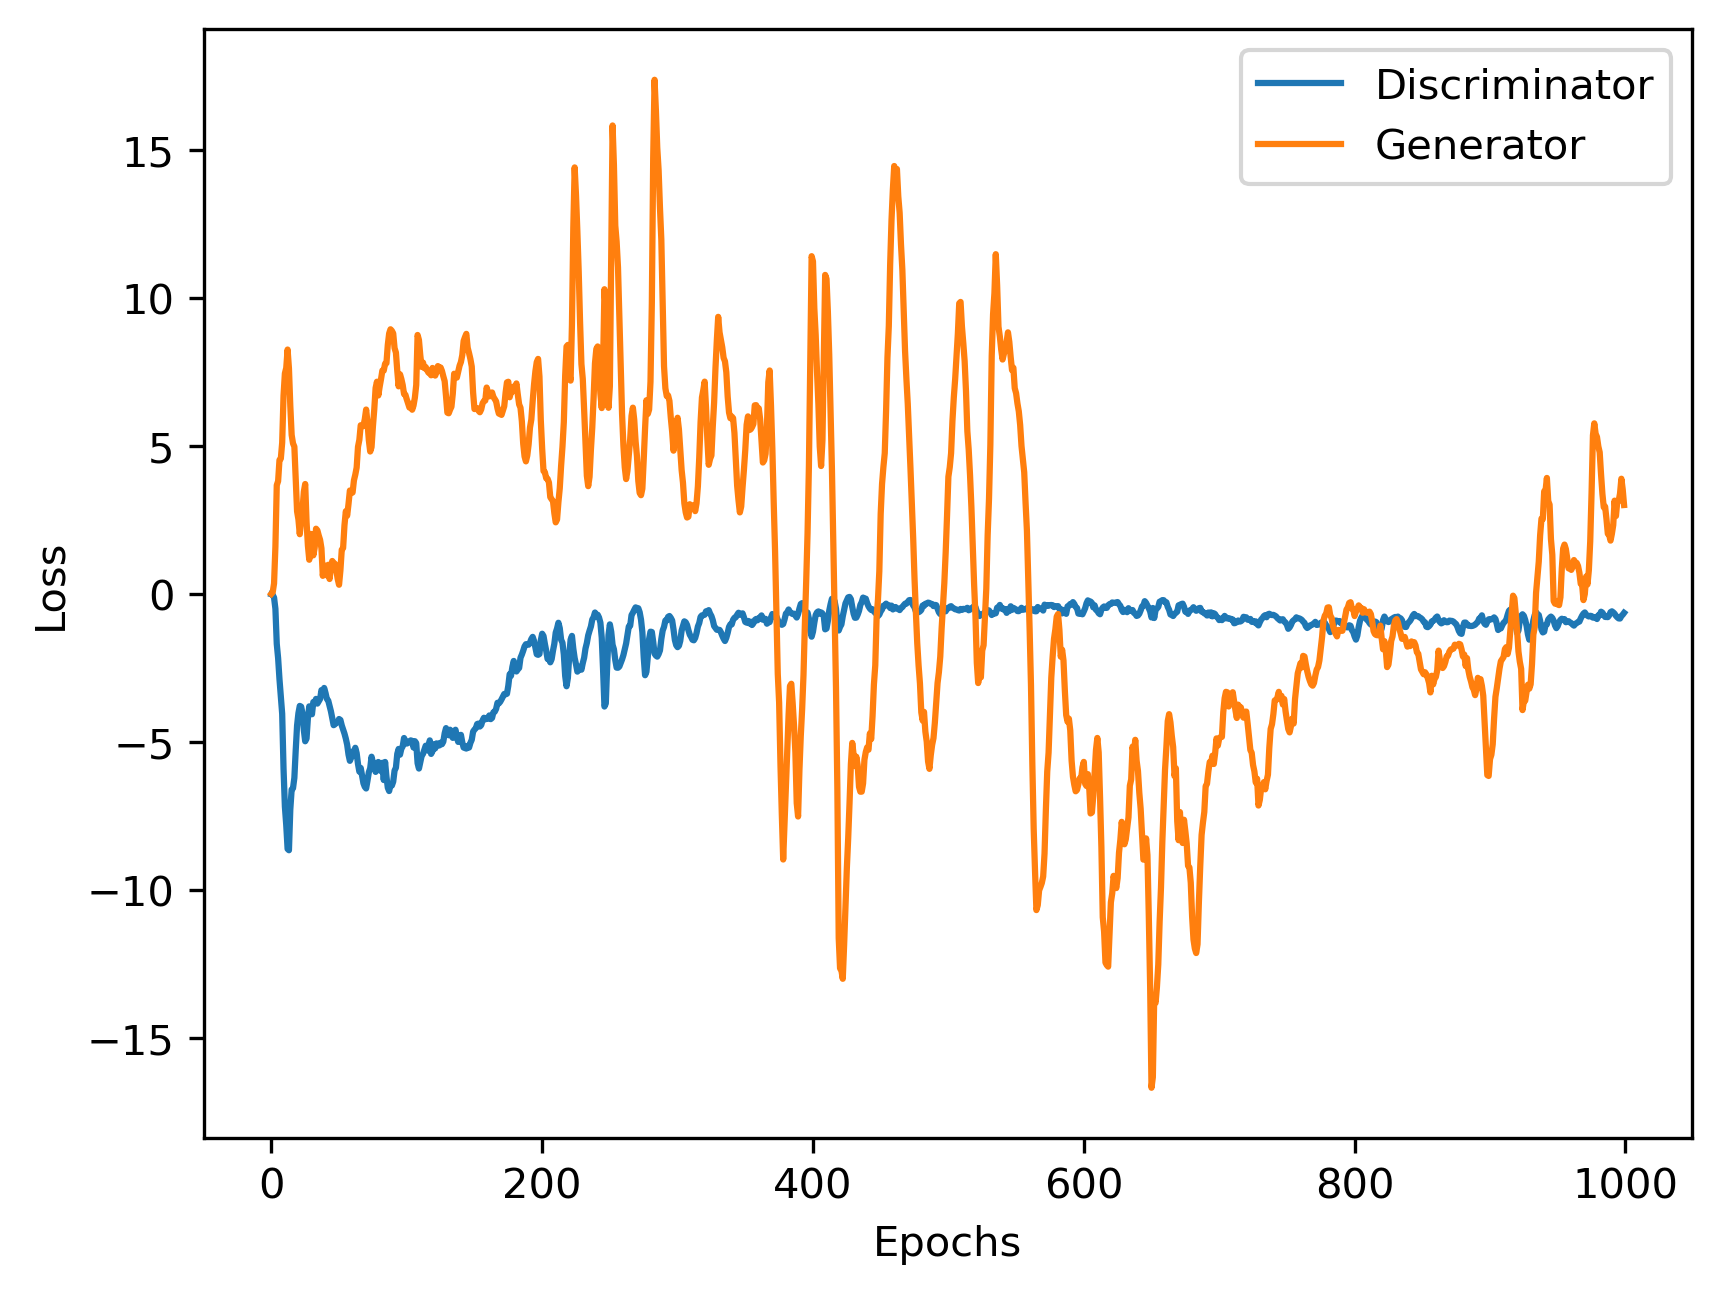
\includegraphics[width=0.45\textwidth]{loss_plots/wpgan_flute_hist_pitch_0729.png}
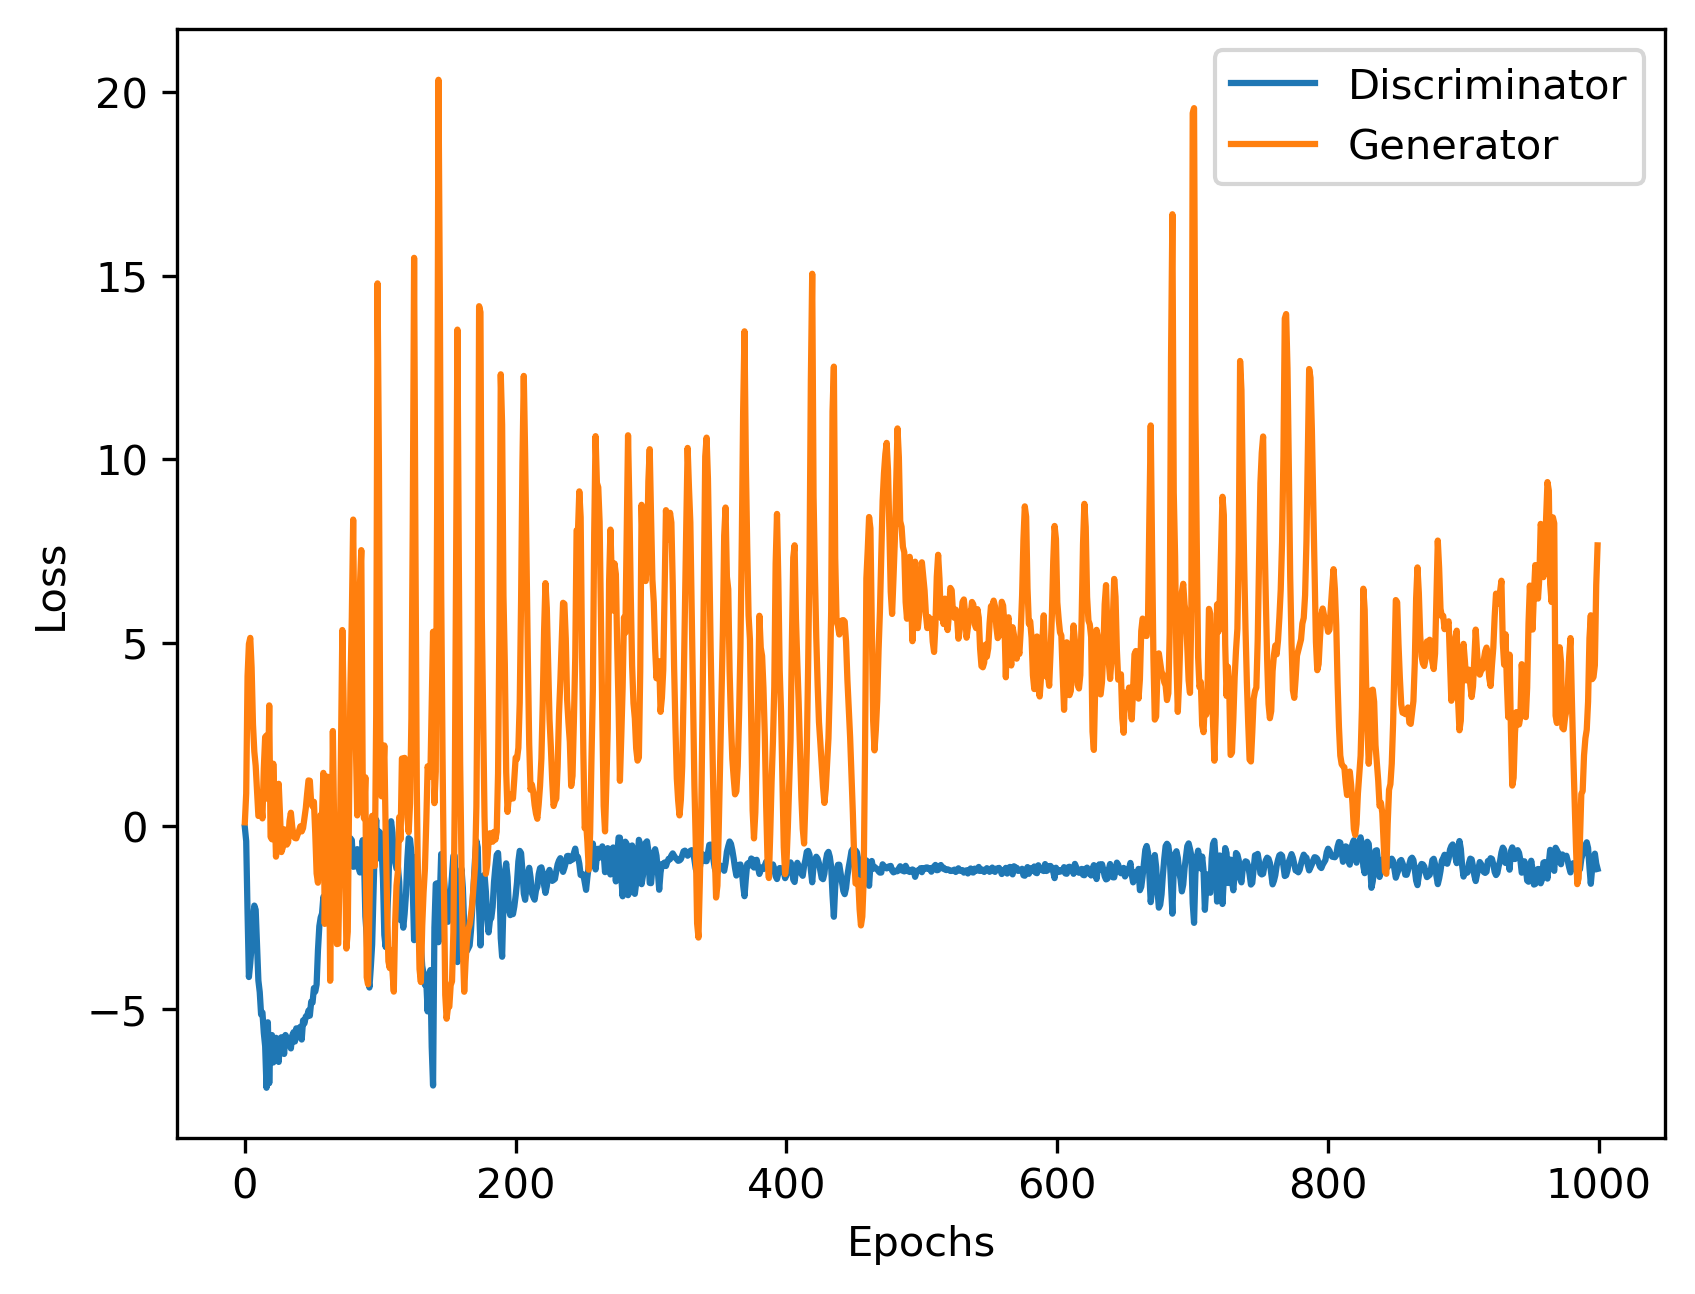
\includegraphics[width=0.45\textwidth]{loss_plots/wpgan_flute_hist_upsample_pitch_0729.png}
\caption{Left: Transpose Convolution, Right: Upsample Layer}
\end{figure*}

\begin{figure*}[t]
\centering
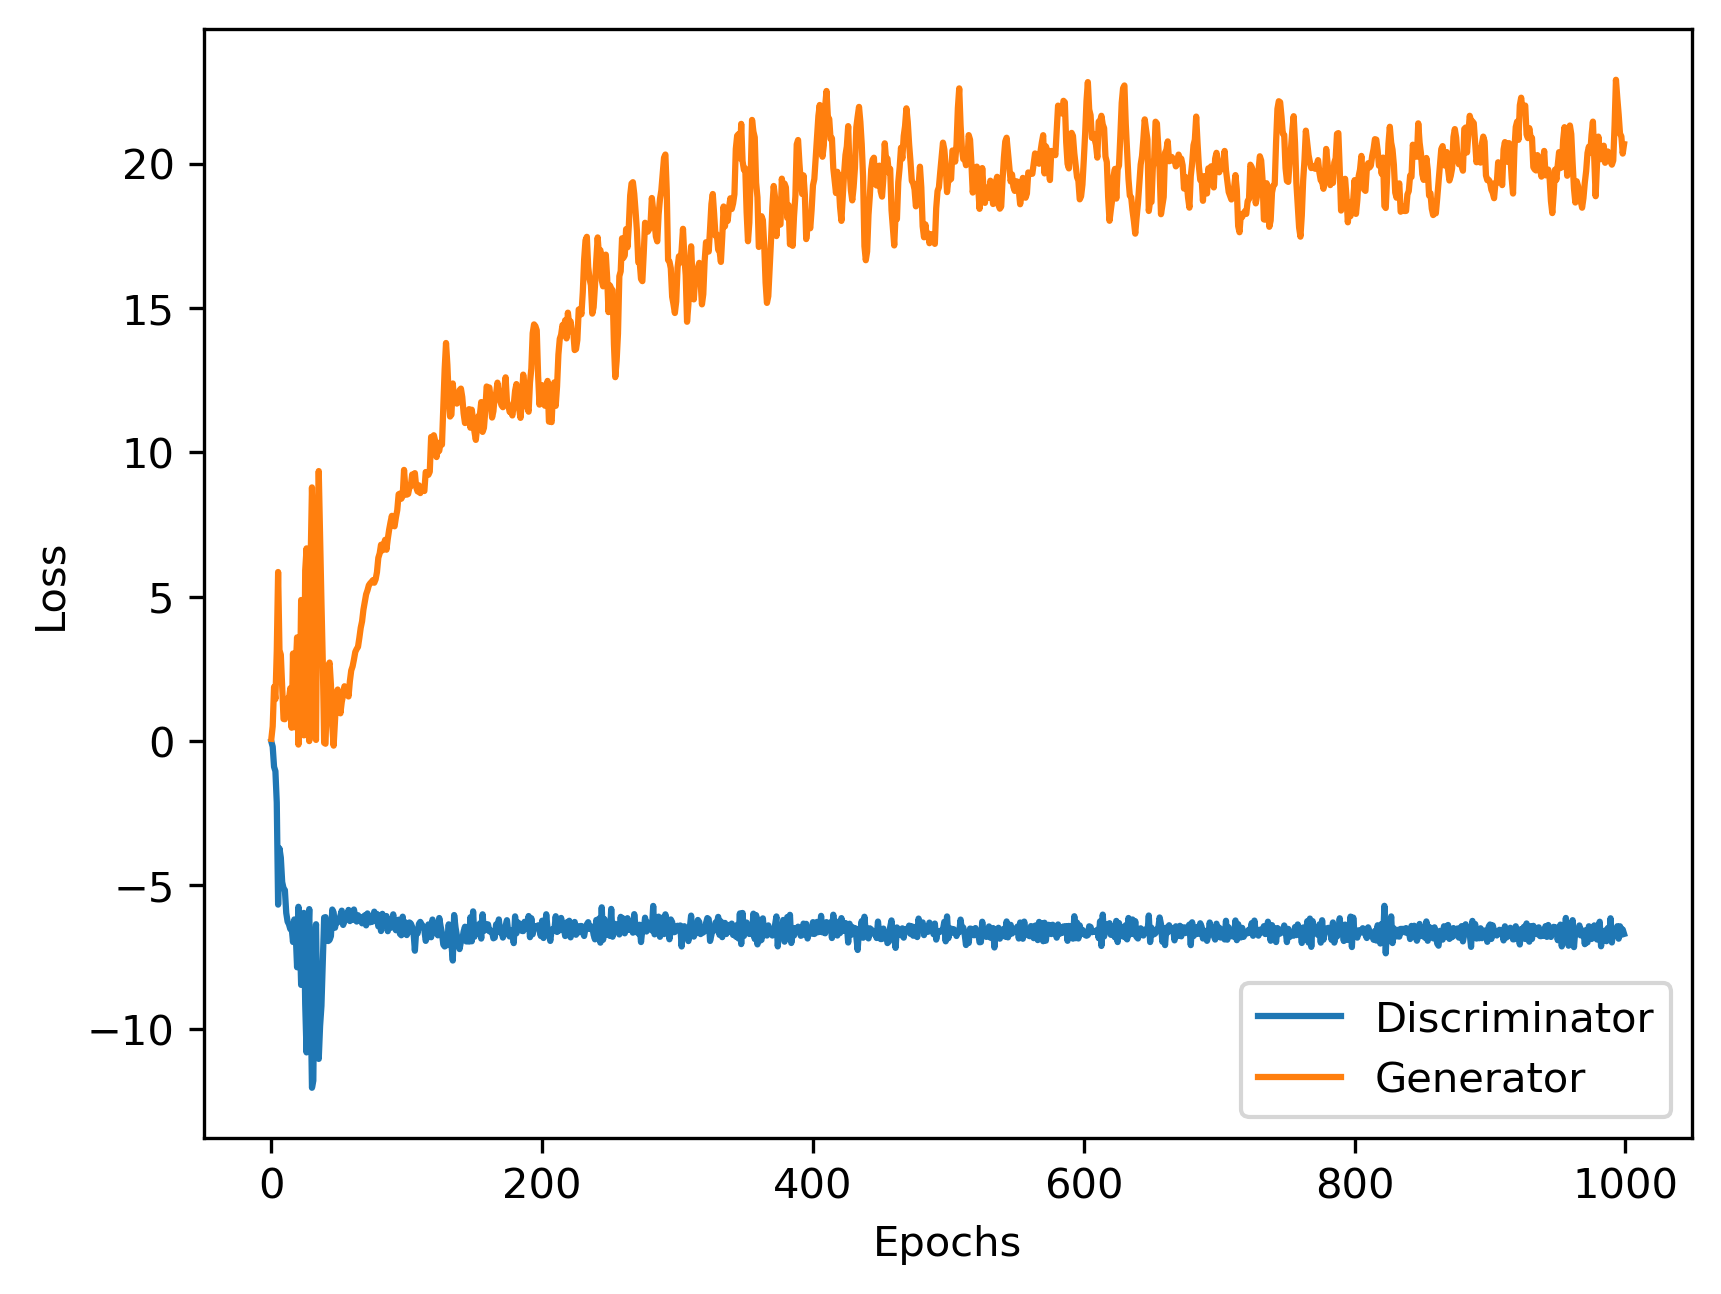
\includegraphics[width=0.45\textwidth]{loss_plots/wpgan_flute_hist_cubic_pitch_0729.png}
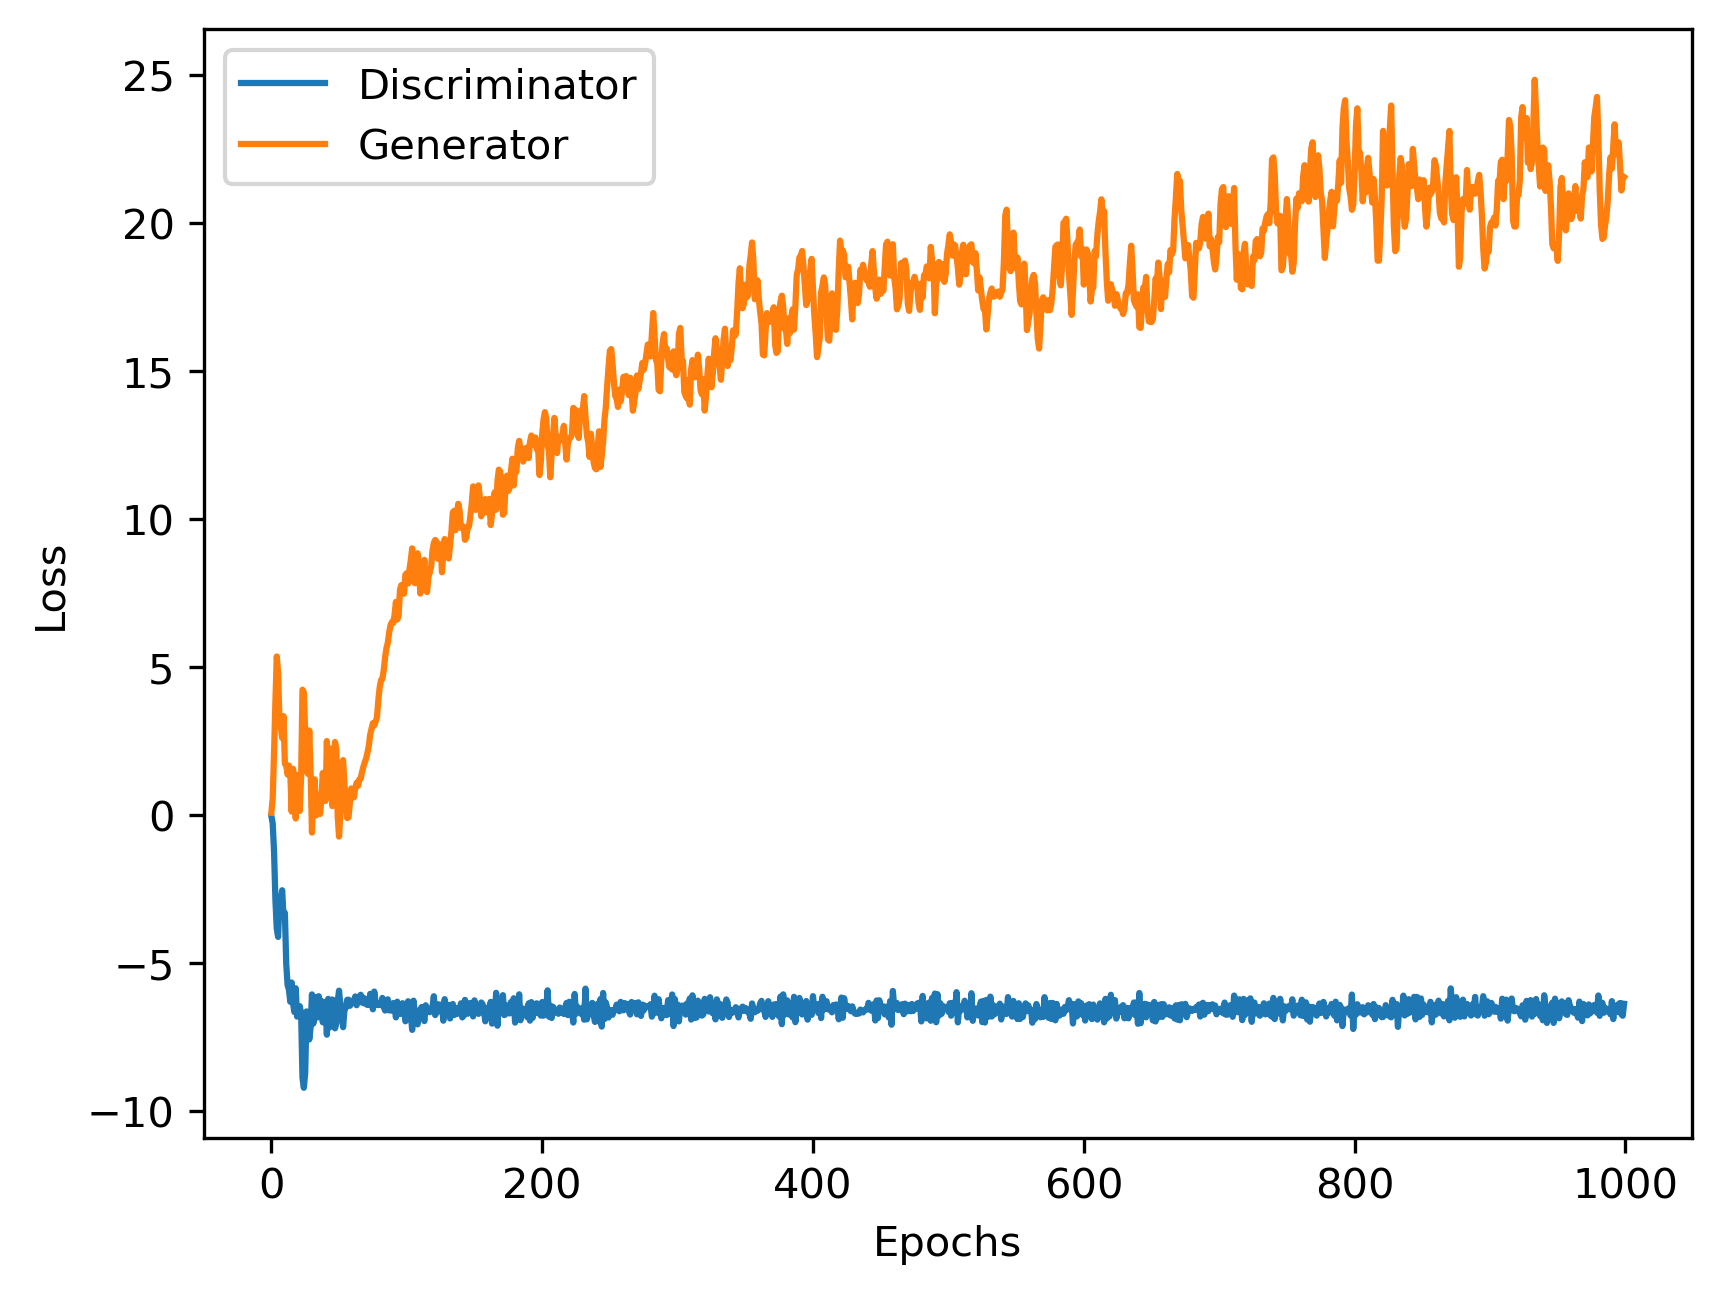
\includegraphics[width=0.45\textwidth]{loss_plots/wpgan_flute_hist_linear_pitch_0729.png}
\caption{Left: Cubic Interpolation, Right: Linear Interpolation}
\end{figure*}

\begin{figure*}[t]
\centering
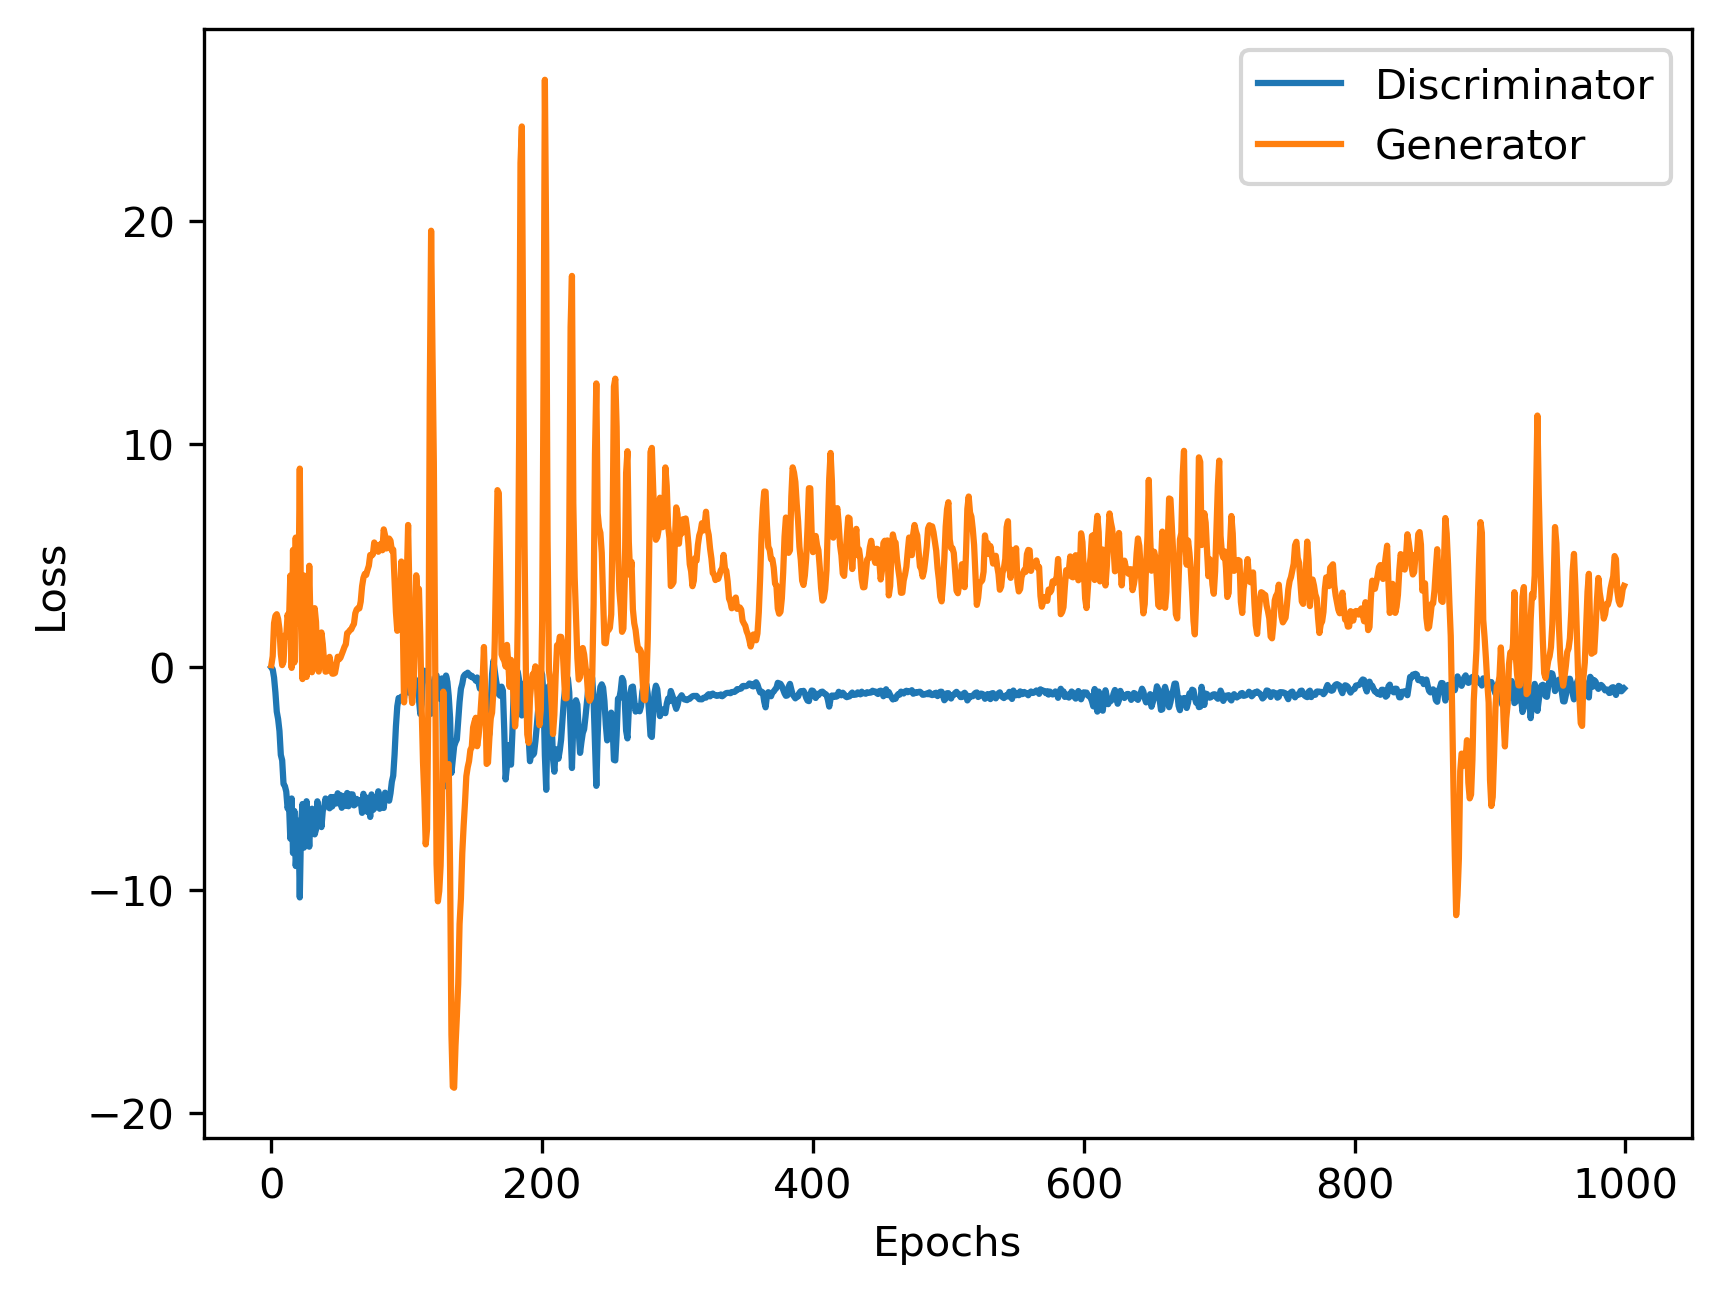
\includegraphics[width=0.45\textwidth]{loss_plots/wpgan_flute_hist_nearest_pitch_0729.png}
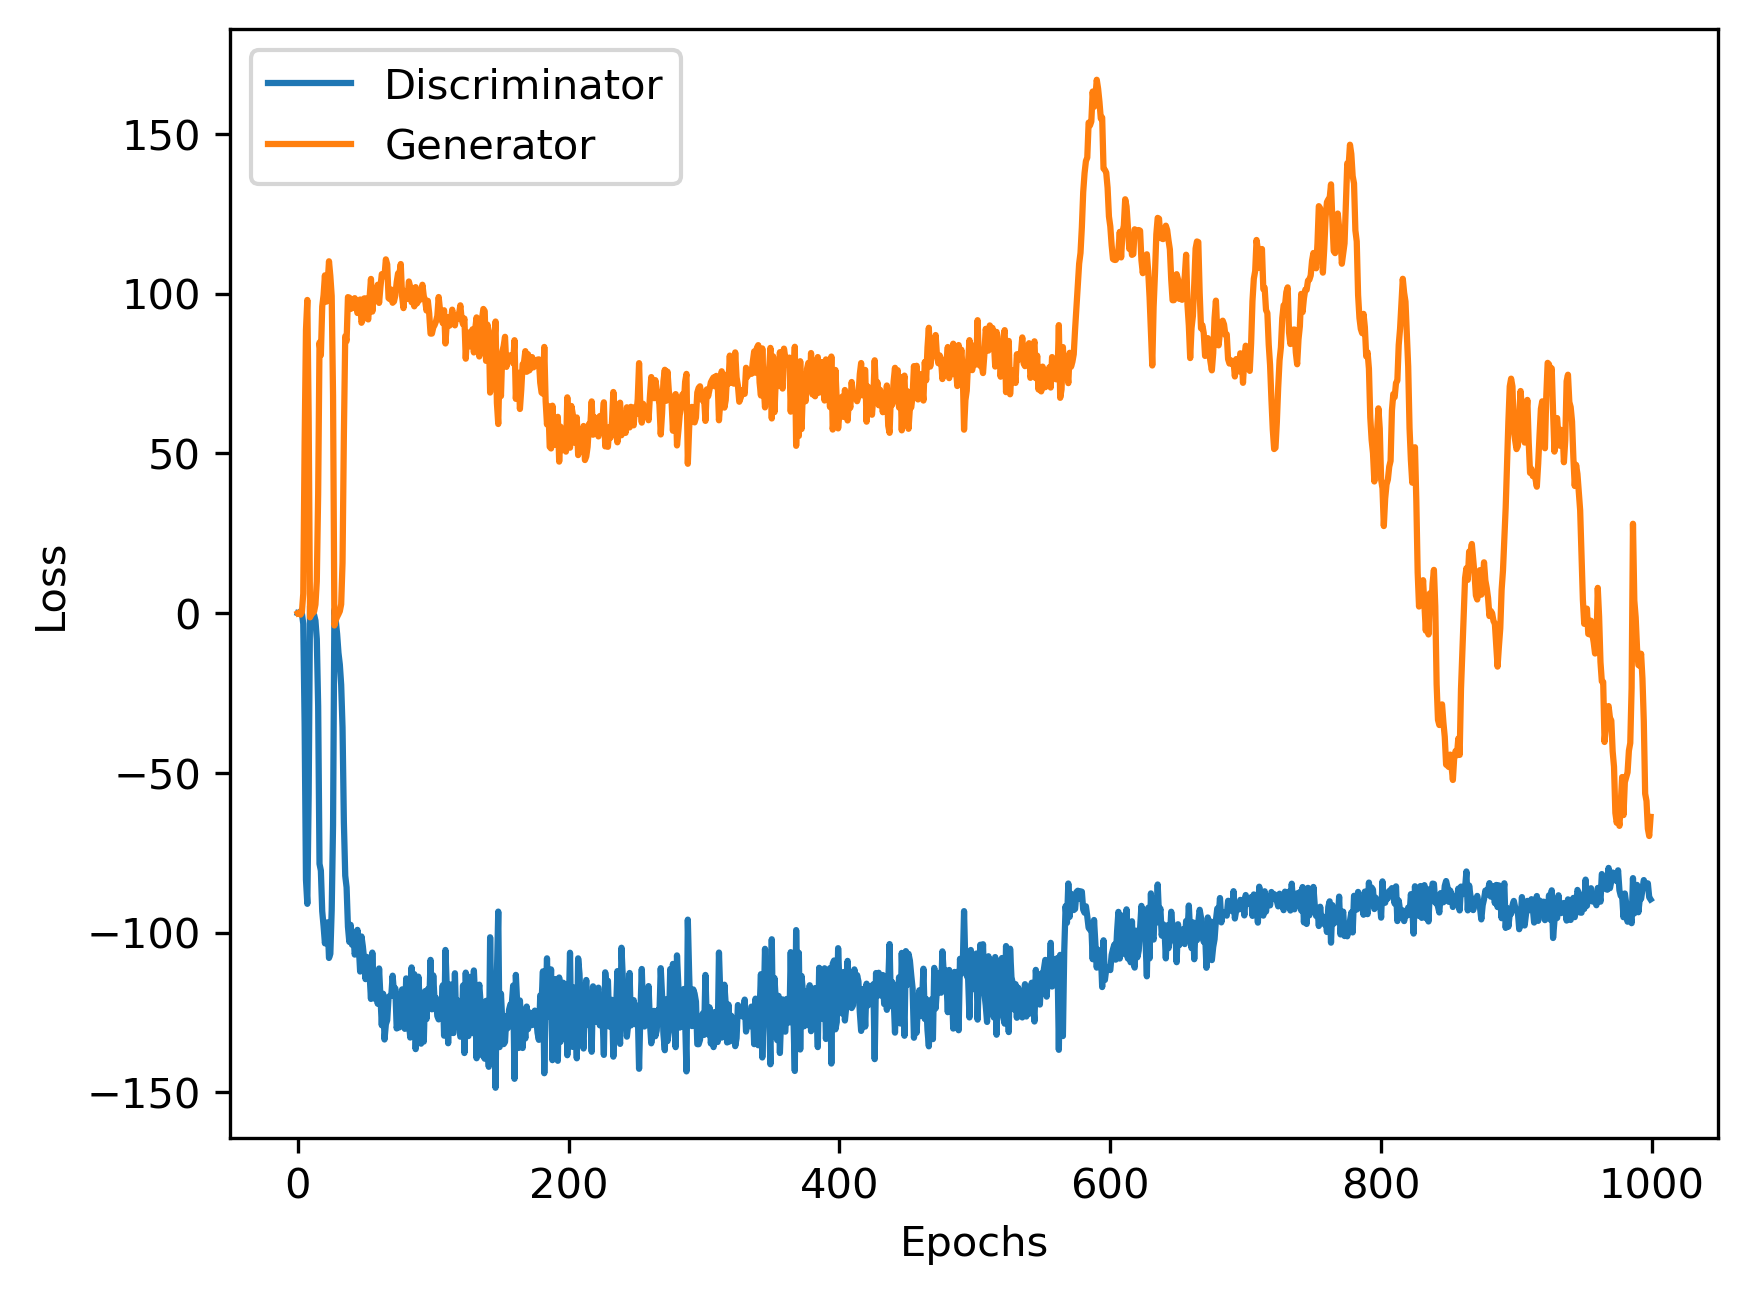
\includegraphics[width=0.45\textwidth]{loss_plots/wpgan_flute_hist_nearest_nonorm_pitch_0729.png}
\caption{Left: Nearest neighbour interpolation, Right: Nearest neighbour interpolation with no batch normalization}
\end{figure*}

\begin{figure*}[t]
\centering
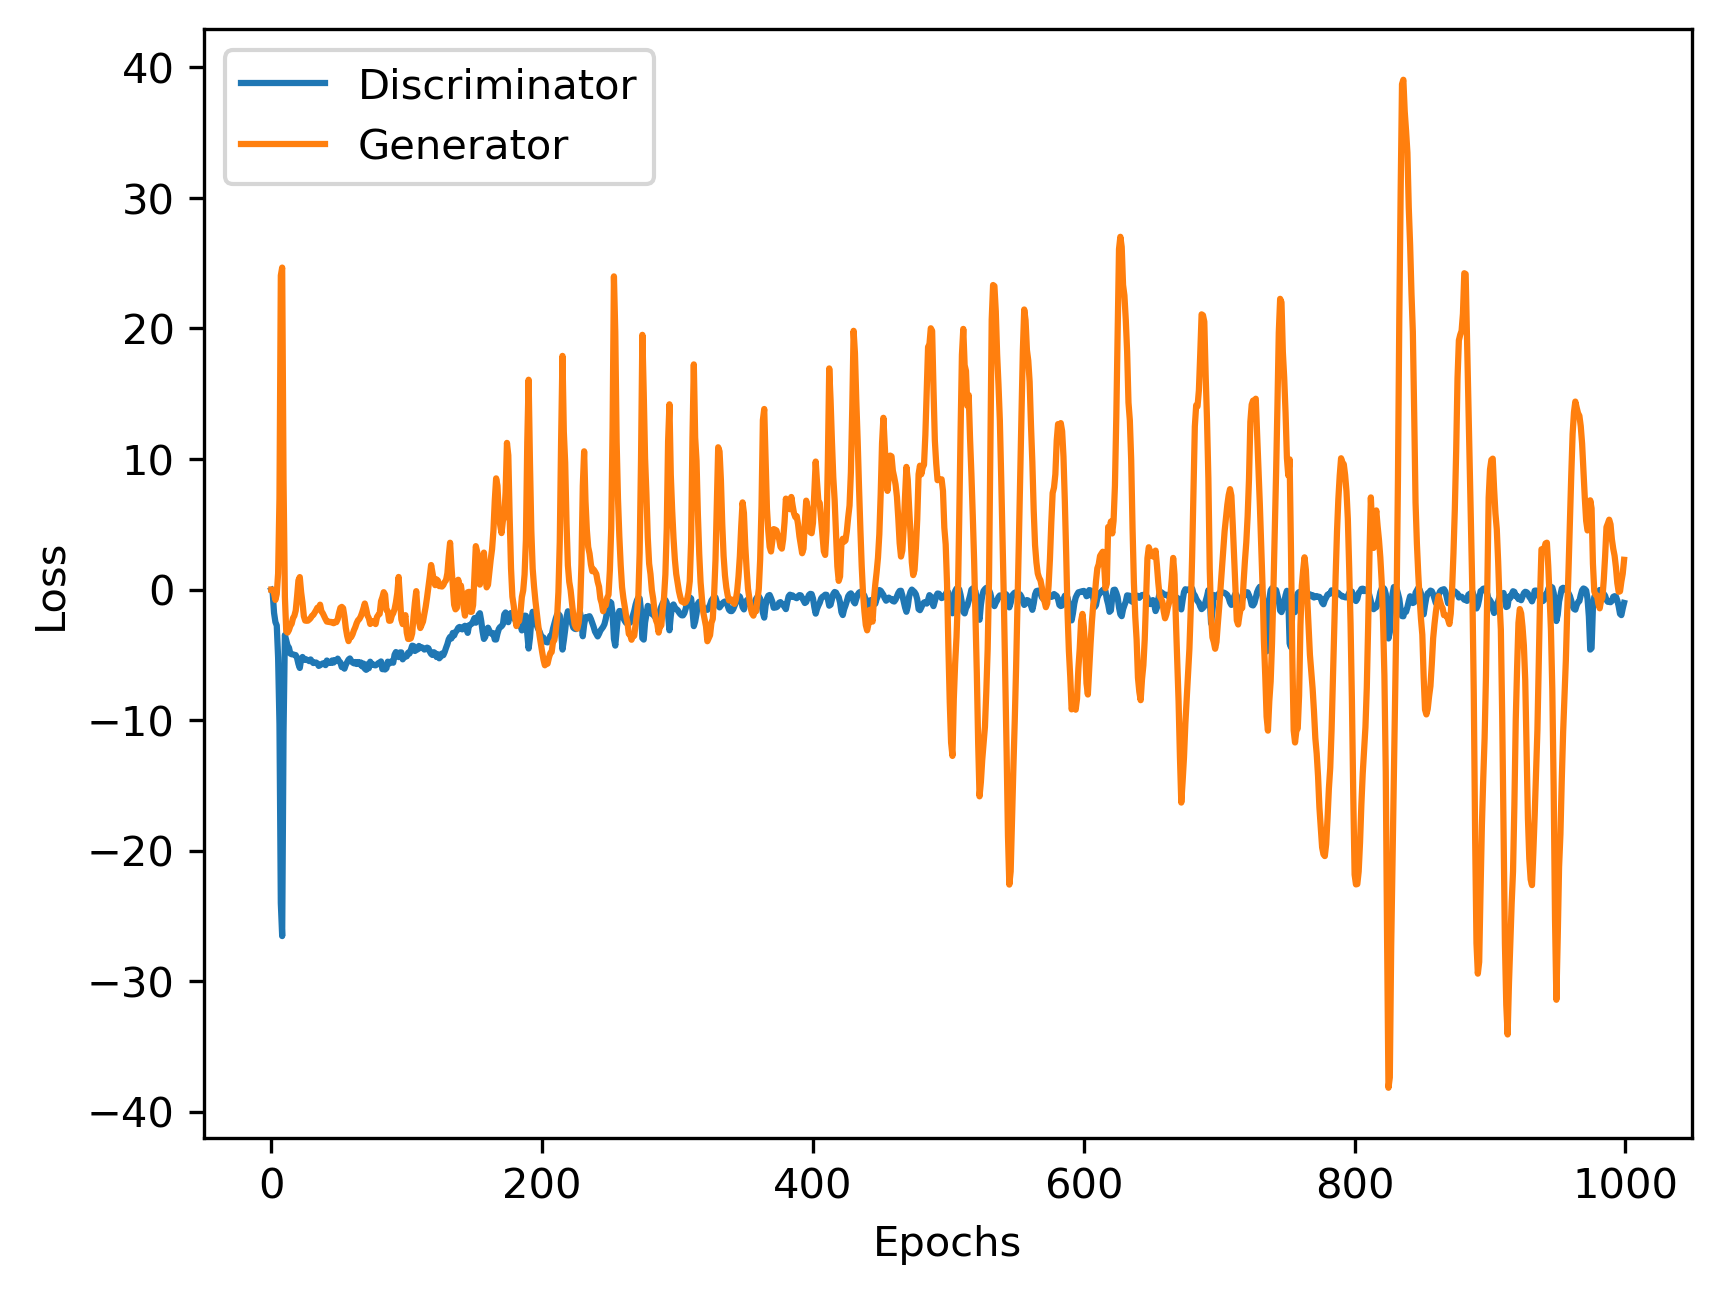
\includegraphics[width=0.45\textwidth]{loss_plots/wpgan_flute_hist_nonorm_pitch_0729.png}
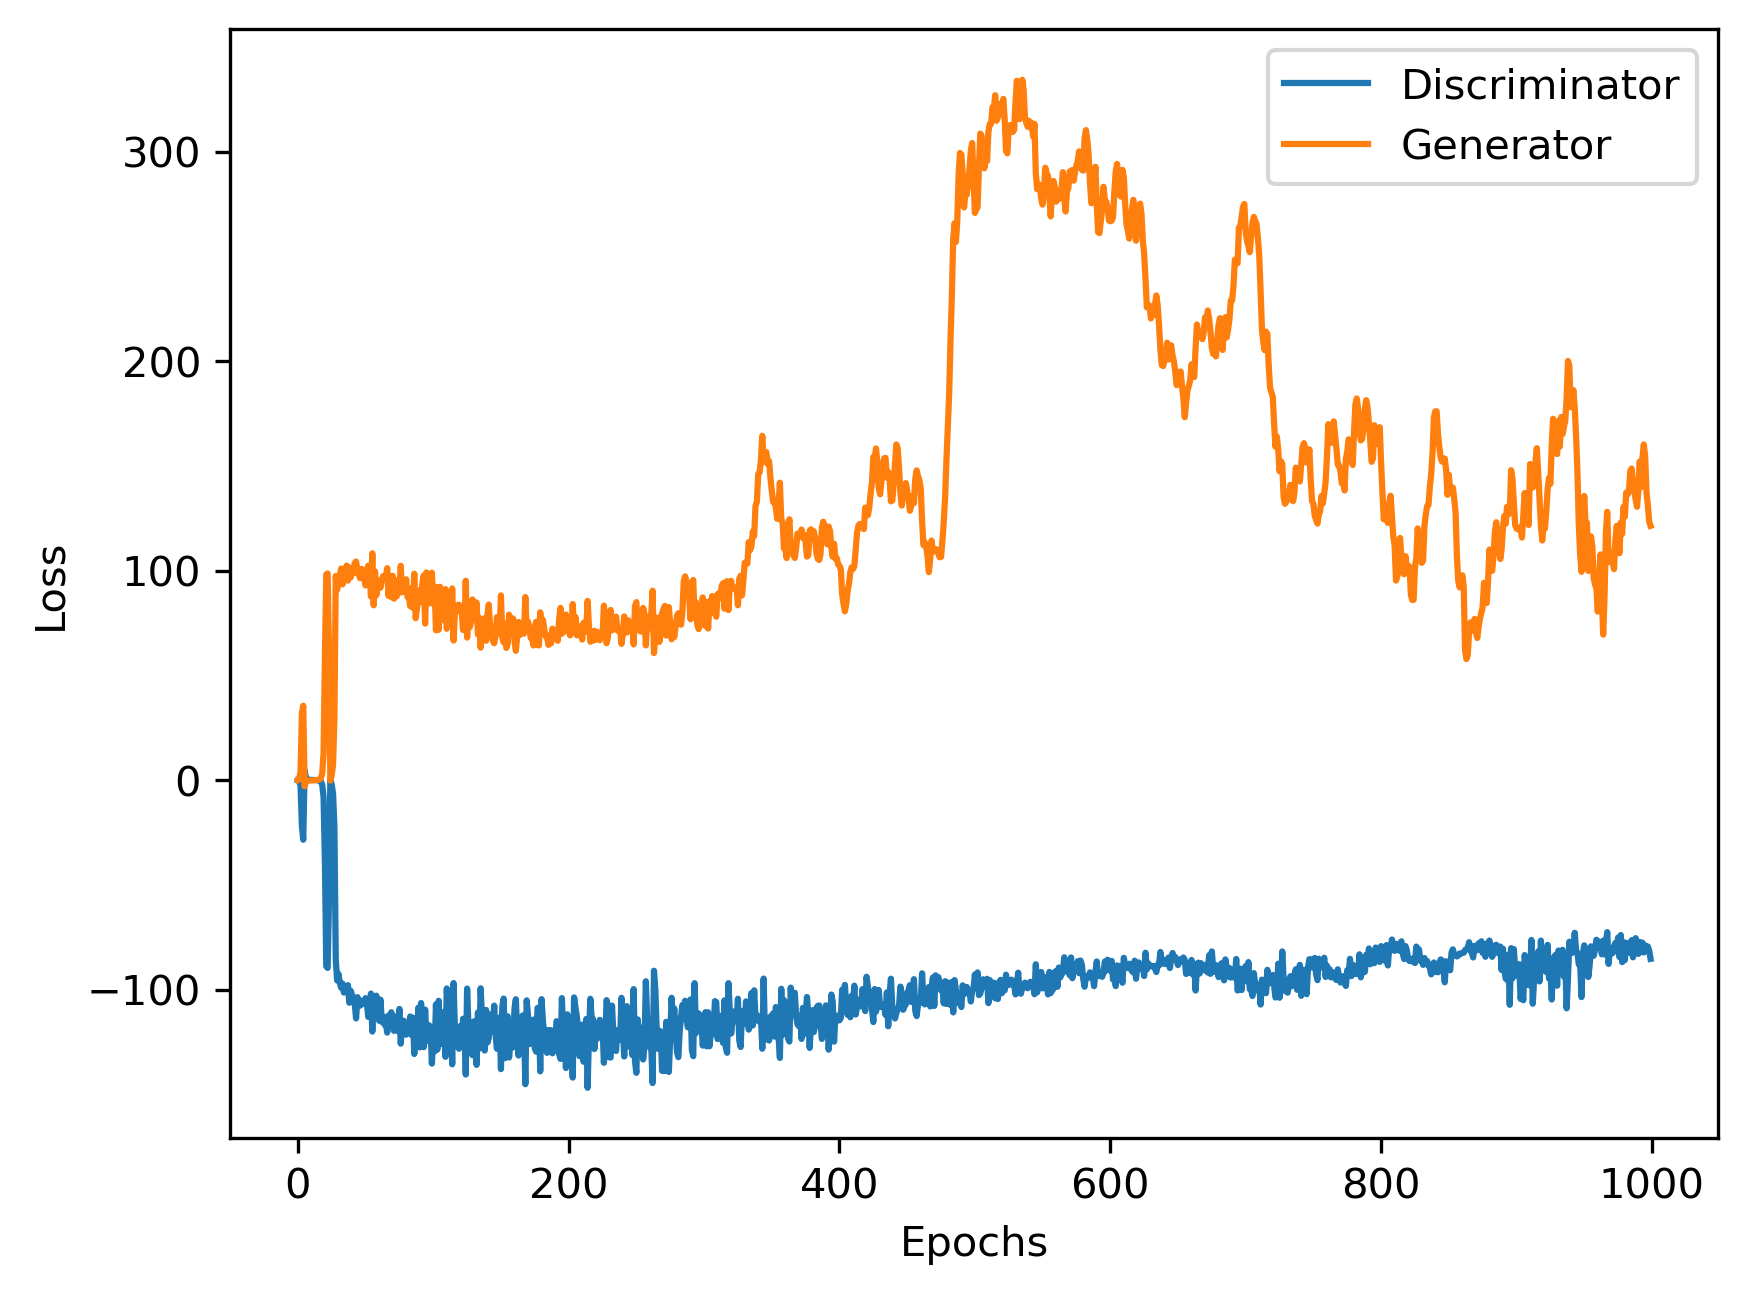
\includegraphics[width=0.45\textwidth]{loss_plots/wpgan_flute_hist_upsample_nonorm_pitch_0729.png}
\caption{Left: Transpose convolution with no batch normalization, Right: Upsample layer with no batch normalization}
\end{figure*}

\begin{figure*}[t]
\centering
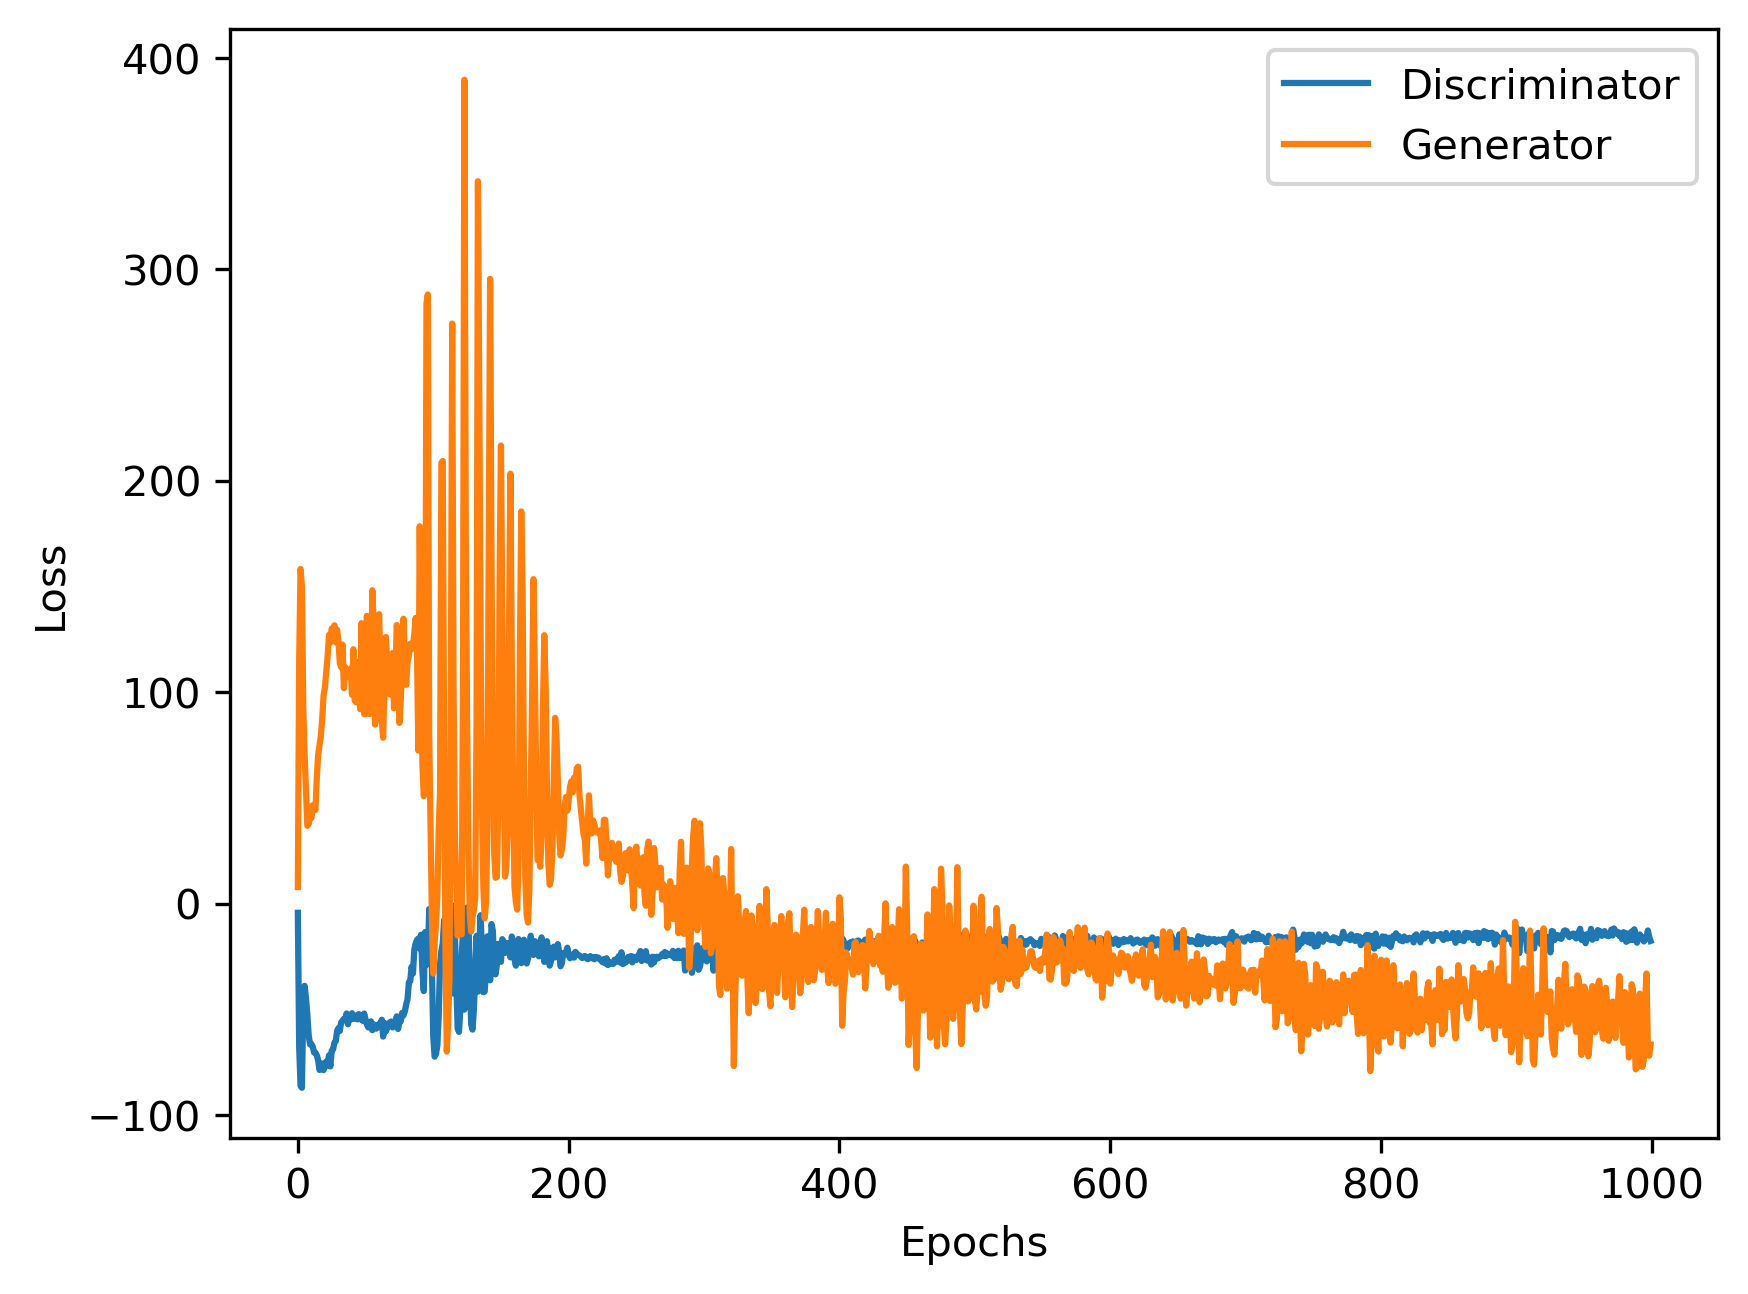
\includegraphics[width=0.45\textwidth]{loss_plots/wpgan_flute_hist_nearest_k5_d50_0803.png}
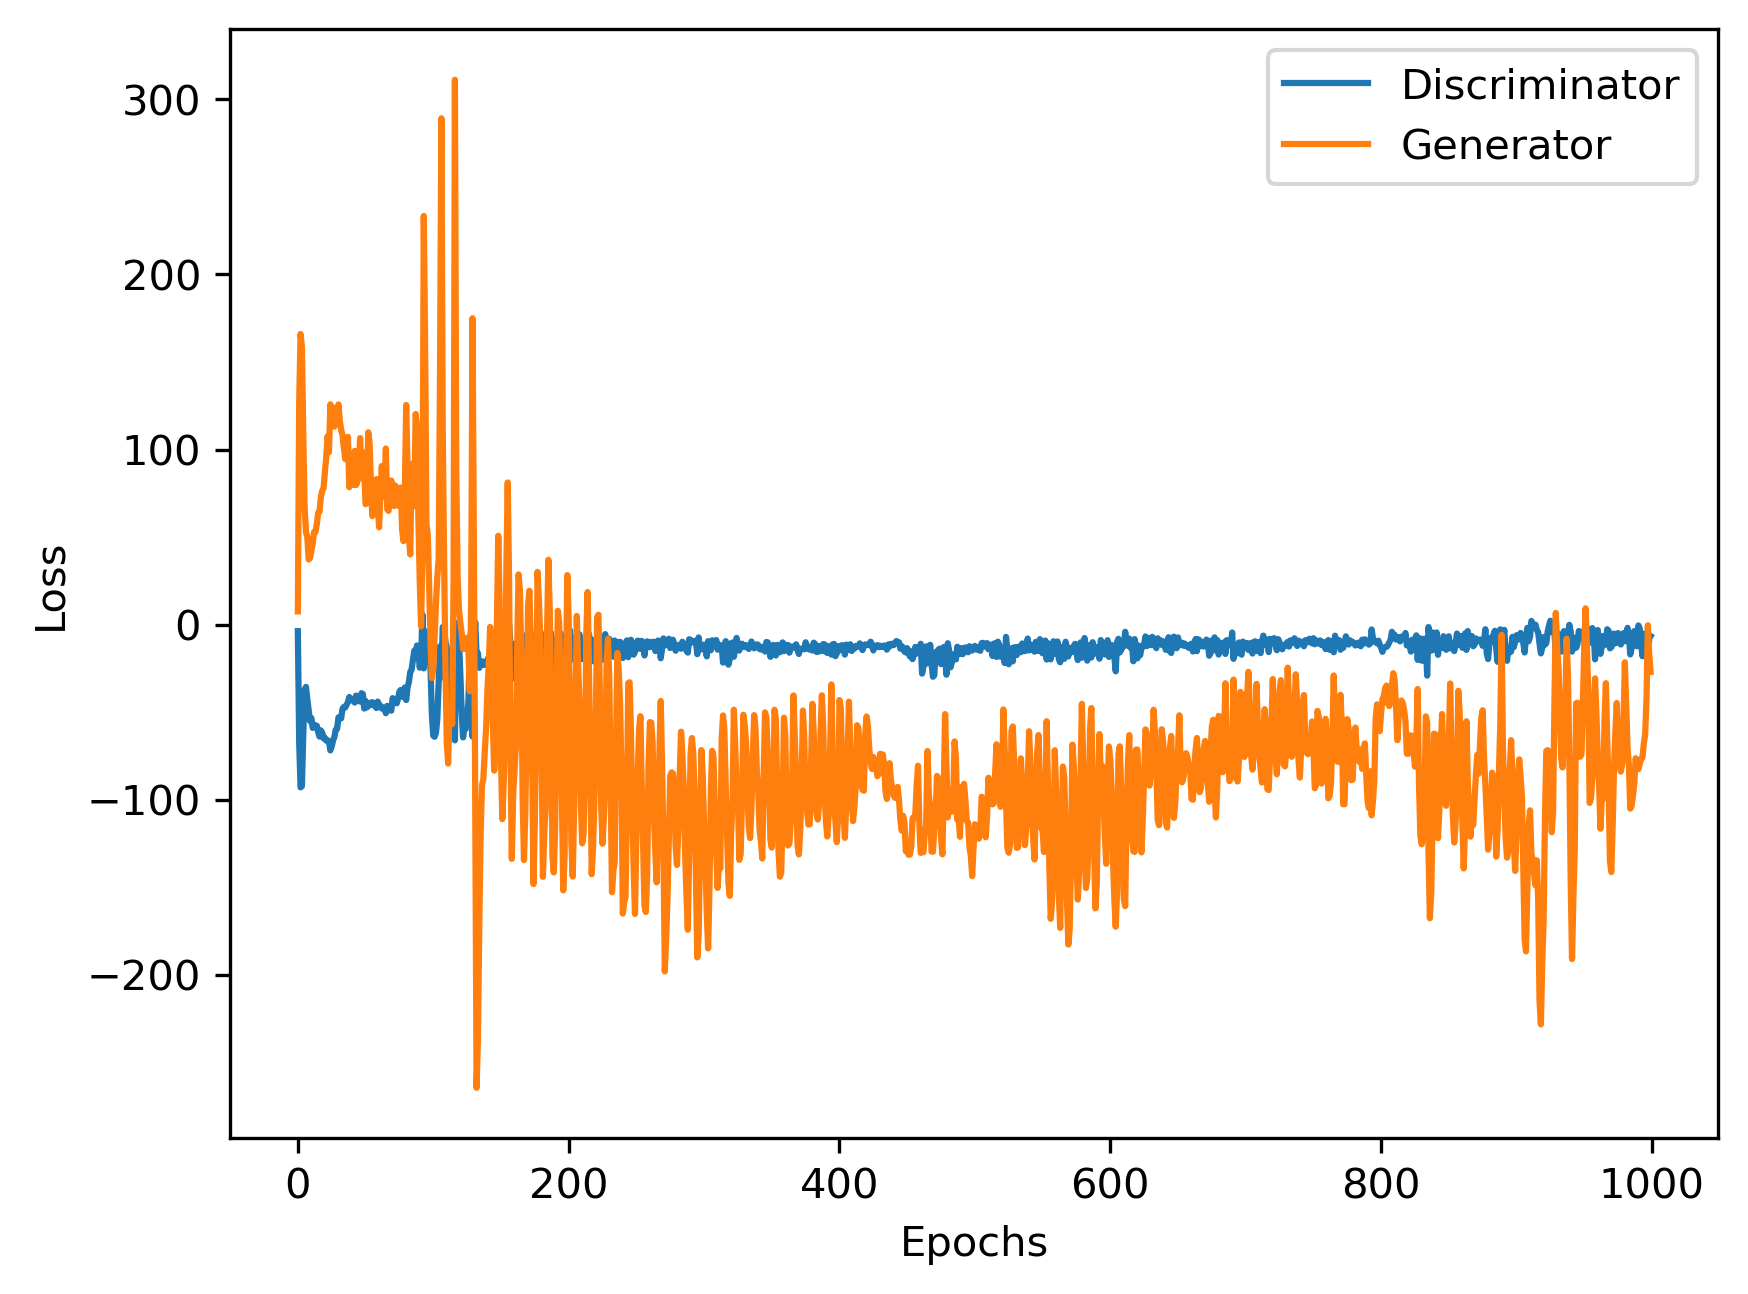
\includegraphics[width=0.45\textwidth]{loss_plots/wpgan_flute_hist_nearest_ps_k5_d50_0803.png}
\caption{Left: Nearest neighbour interpolation and a dropout of 50\% in the generator. Right: Nearest neighbour interpolation, dropout of 50\% in the generator, and phase shuffling.}
\end{figure*}

\begin{figure*}[t]
\centering
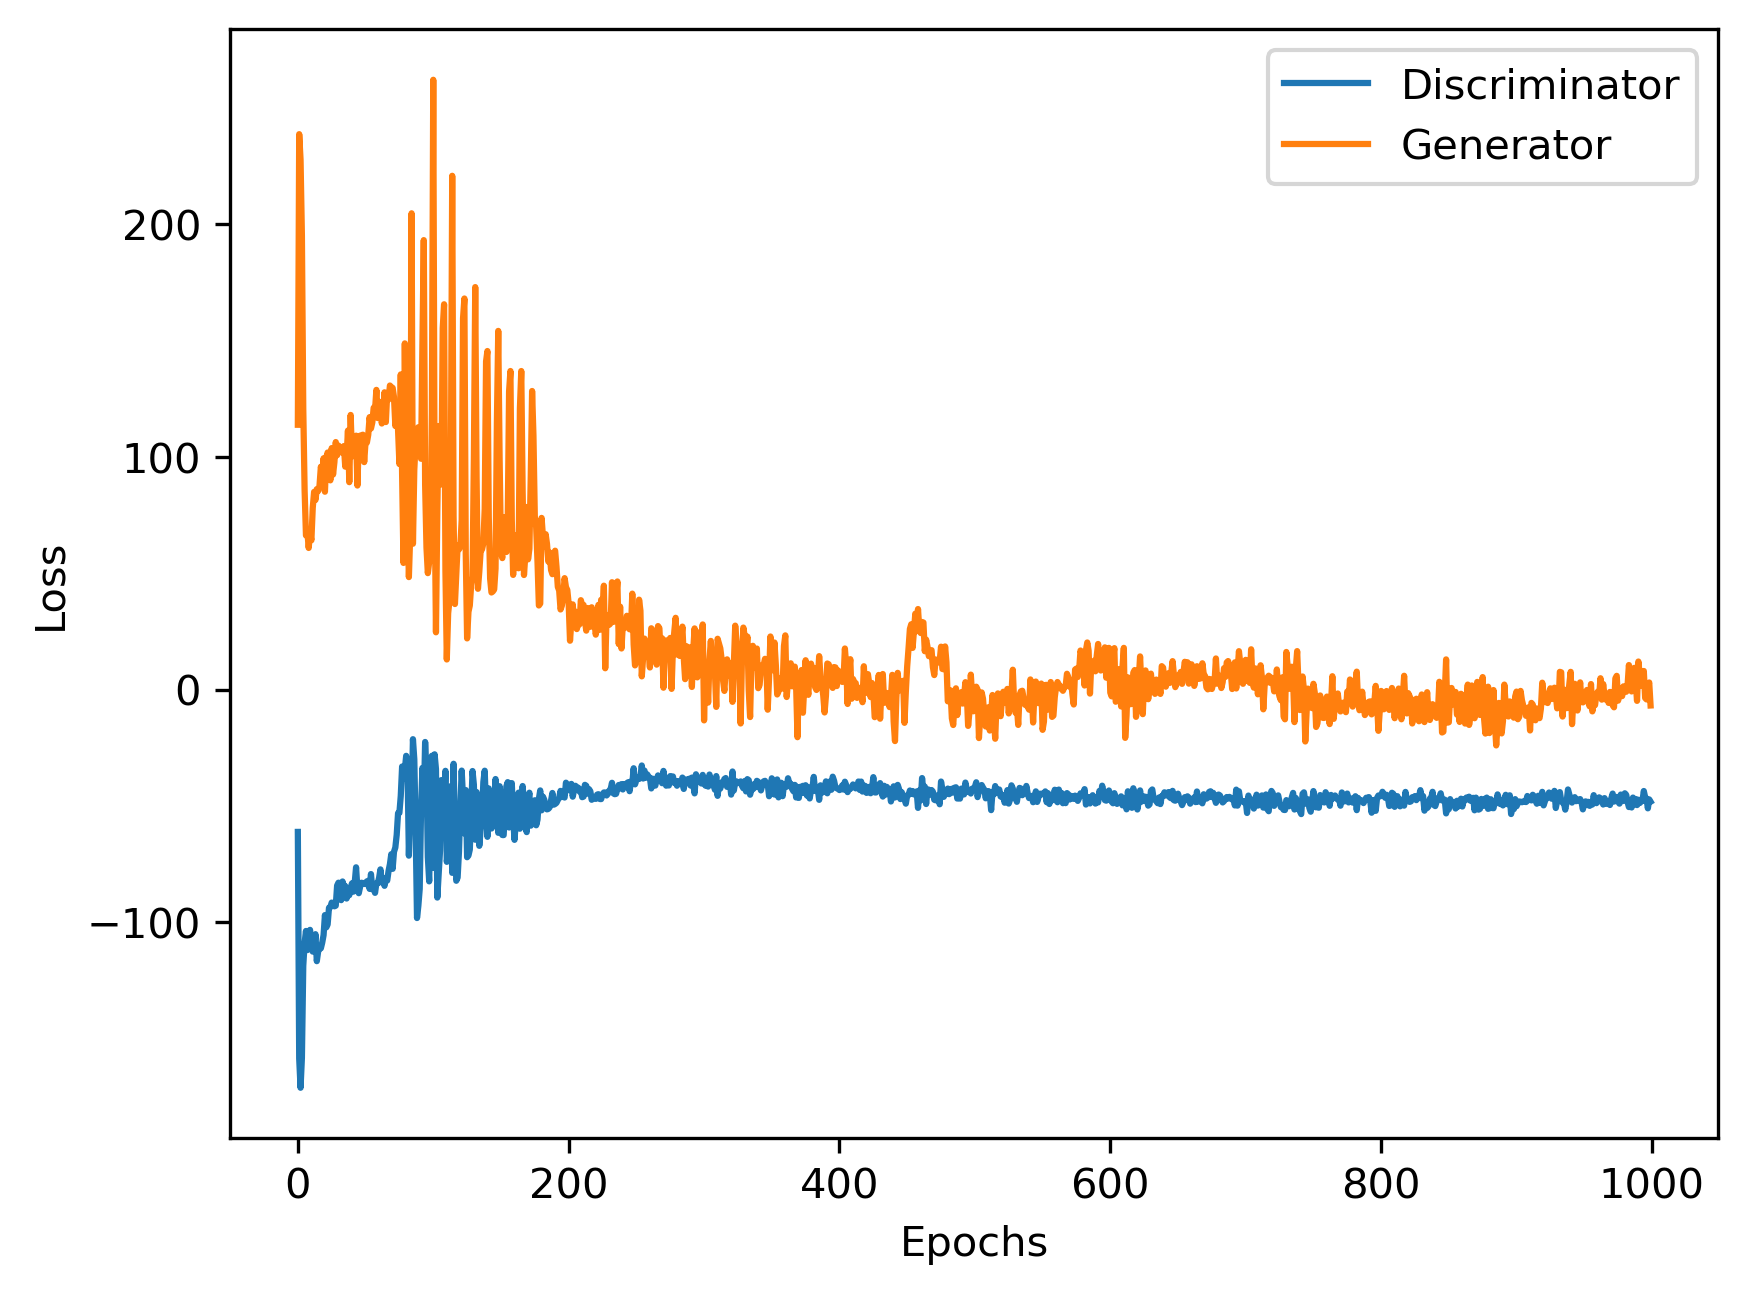
\includegraphics[width=0.45\textwidth]{loss_plots/wpgan_flute_hist_nearest_k15_d50_0803.png}
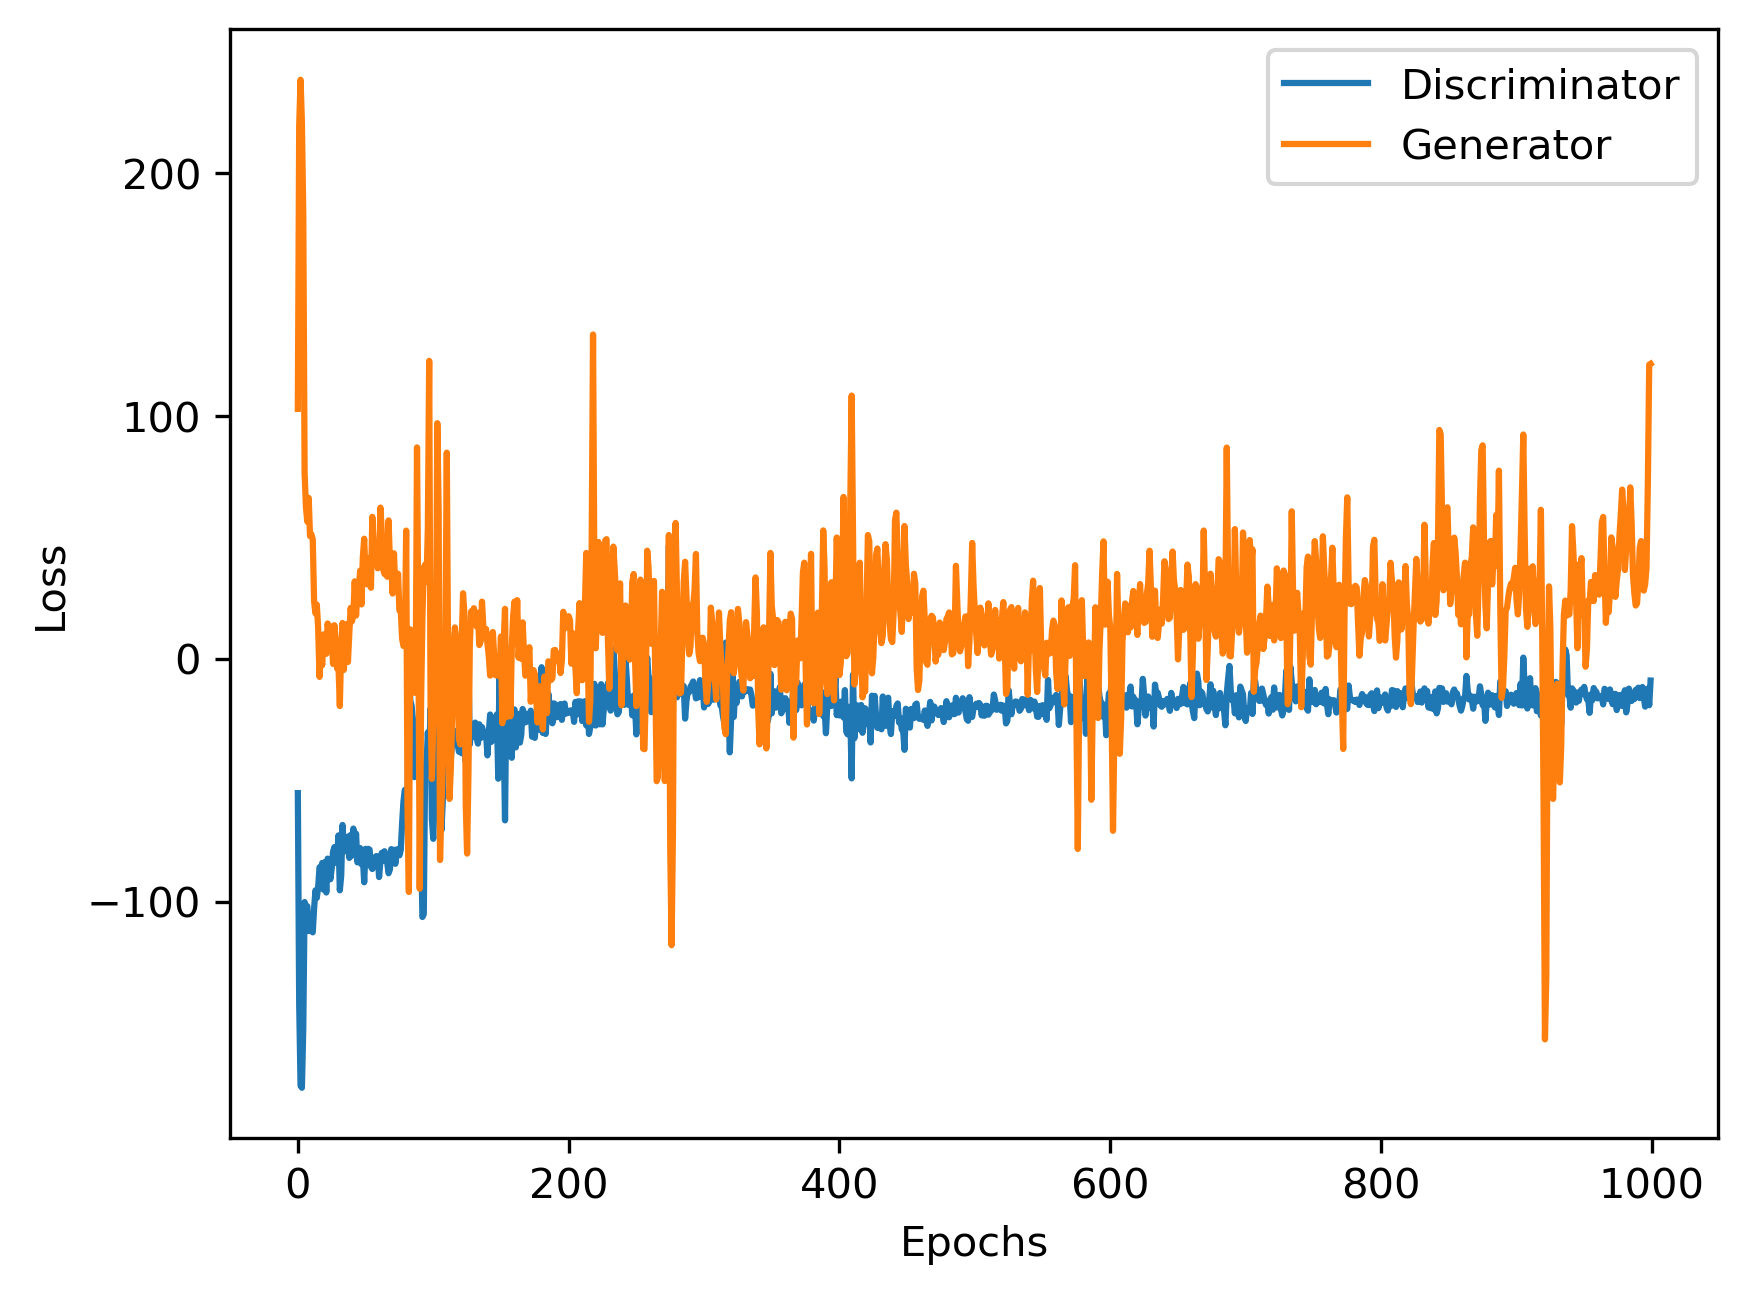
\includegraphics[width=0.45\textwidth]{loss_plots/wpgan_flute_hist_nearest_ps_k15_d50_0803.png}
\caption{Left: Nearest neighbour interpolation and a dropout of 50\% in the generator, discriminator kernel size of 15. Right: Nearest neighbour interpolation, dropout of 50\% in the generator, phase shuffling, and discriminator kernel size of 15}
\end{figure*}

\begin{figure*}[t]
\centering
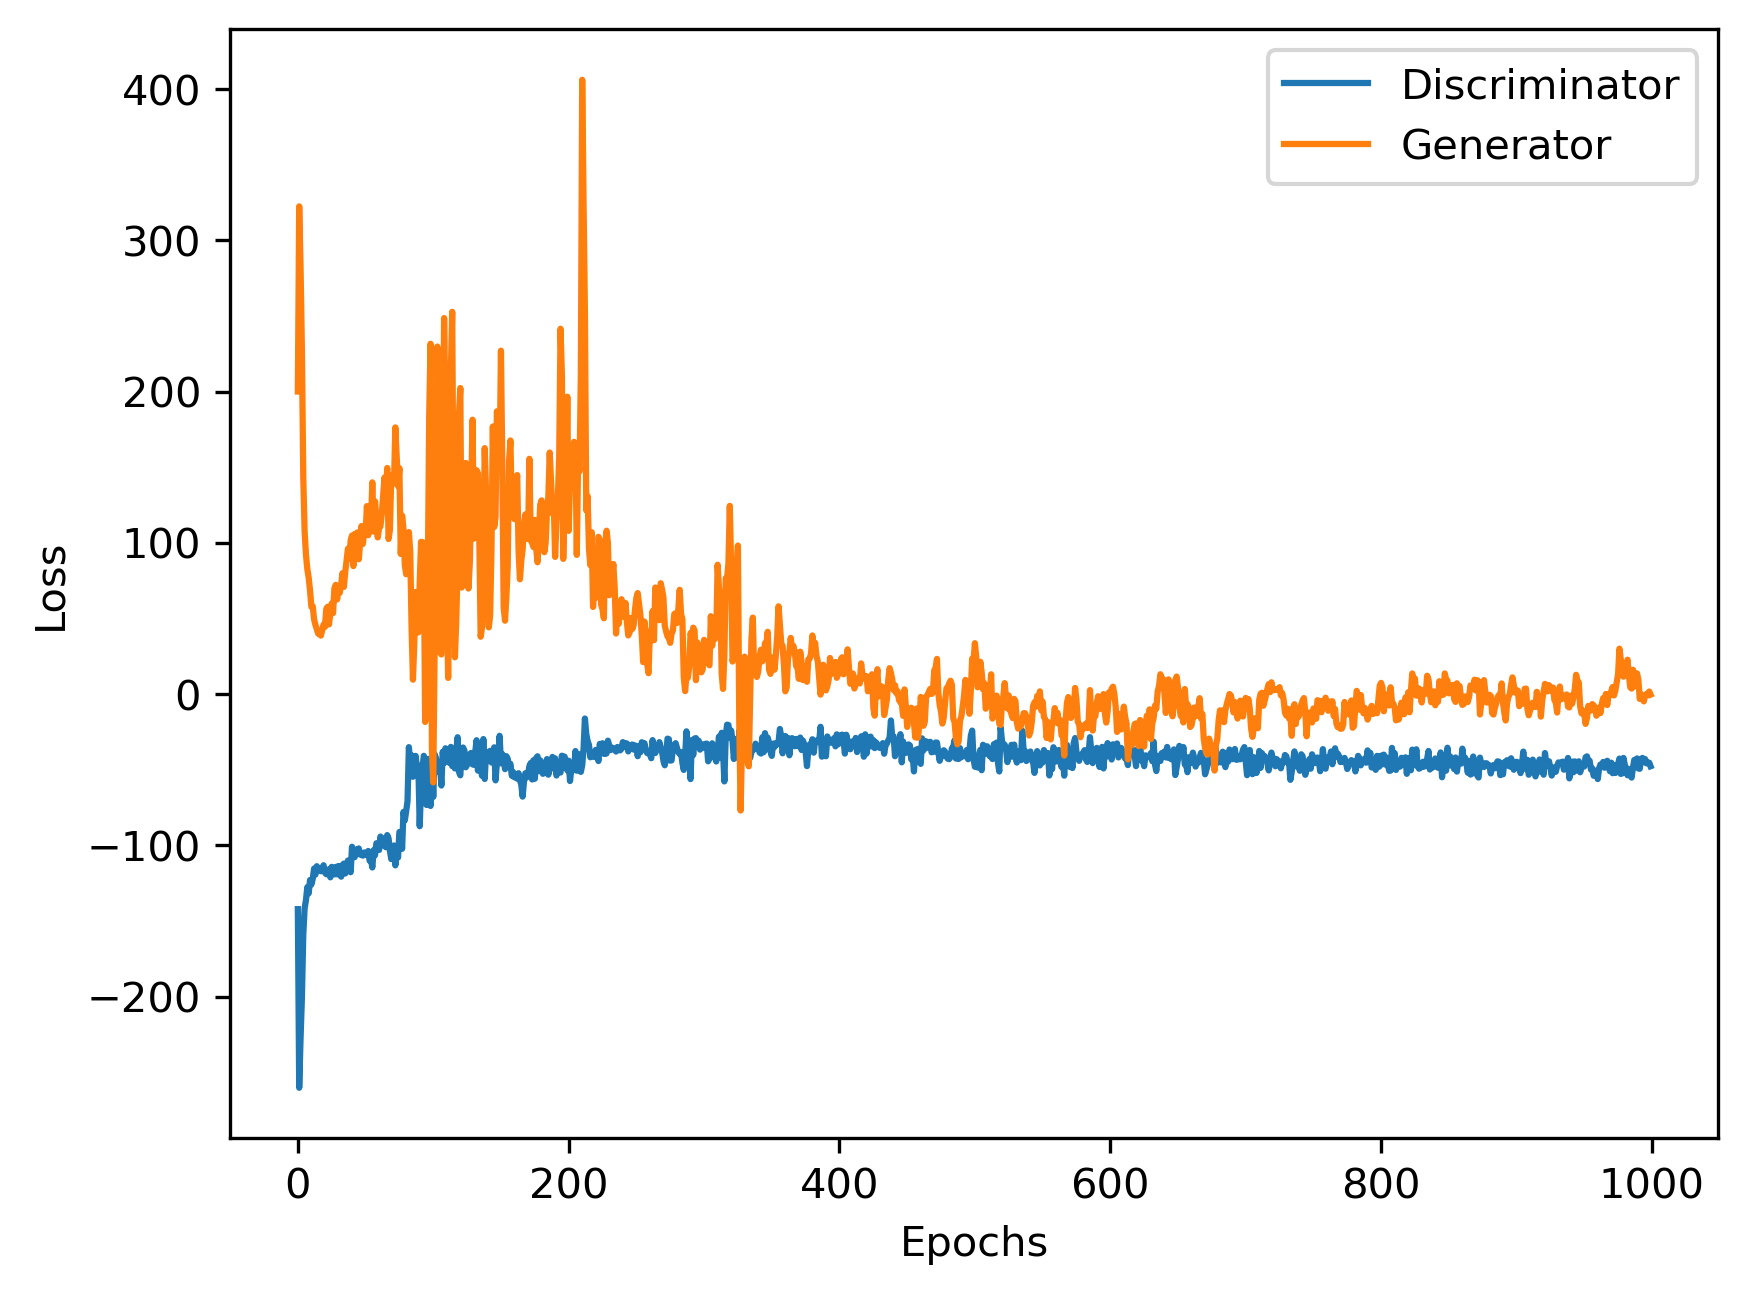
\includegraphics[width=0.45\textwidth]{loss_plots/wpgan_flute_hist_nearest_d50_0803.png}
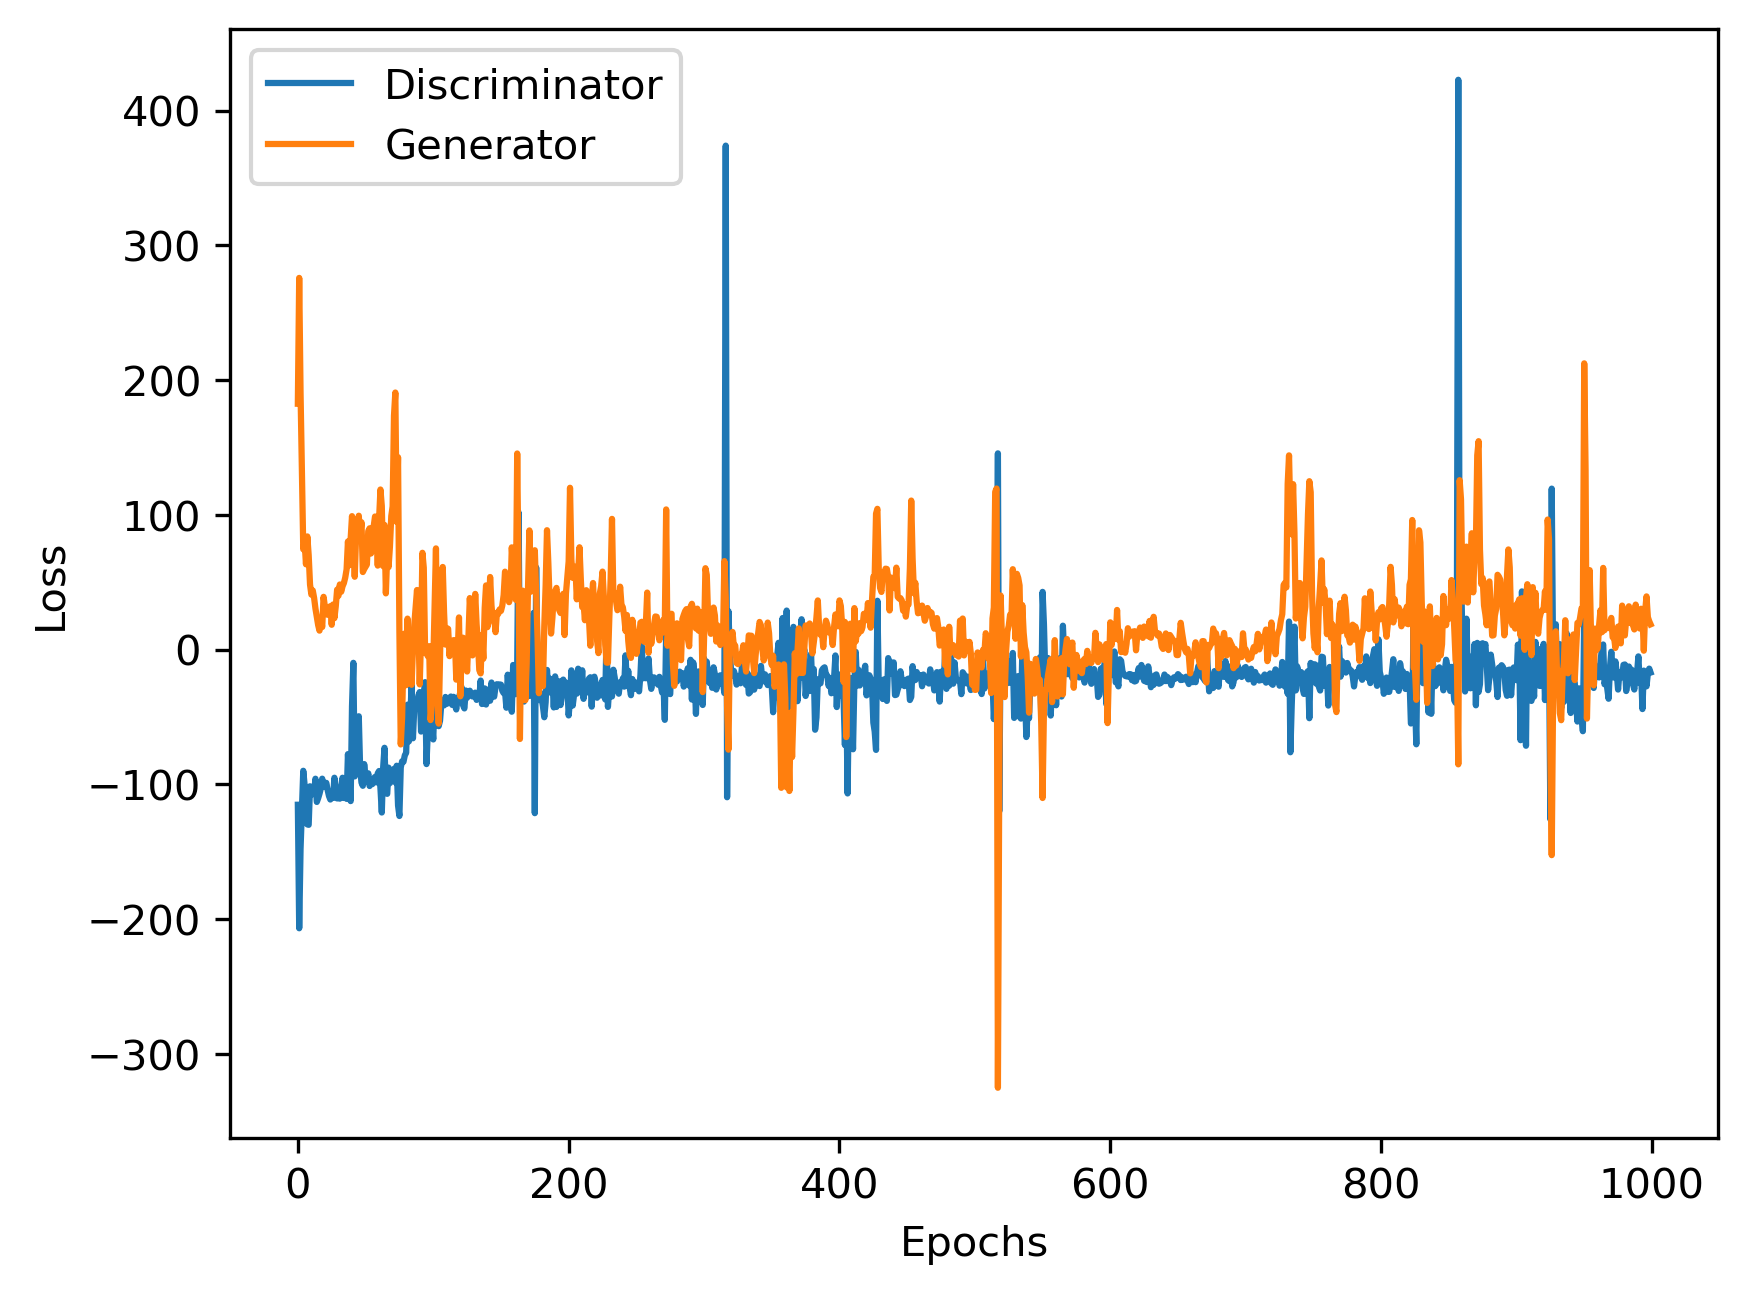
\includegraphics[width=0.45\textwidth]{loss_plots/wpgan_flute_hist_nearest_ps_d50_0803.png}
\caption{Left: Nearest neighbour interpolation and a dropout of 50\% in the generator, discriminator kernel size of 25. Right: Nearest neighbour interpolation, dropout of 50\% in the generator, phase shuffling, and discriminator kernel size of 25}
\end{figure*}
